%TC:ignore
\documentclass{article}
\usepackage{graphicx} % Required for inserting images
\usepackage{hyperref}
\usepackage{lscape}
\usepackage{pdflscape}
%TC:endignore

\title{The genetics of Mitochondrial Dysfunction in Sporadic Parkinson's disease}
\author{Thomas Brightwell; Supervisors: Toby Andrew and Rahel Feleke}

\date{August 22nd 2024}

\begin{document}

\maketitle
This project
report is submitted in partial fulfilment of the requirements for award of MSc in Human Molecular
Genetics, Imperial College London. I hereby confirm that it is an original work, representing my
own academic effort and that all sources have been fully acknowledged.
\newpage
\begin{abstract}
\end{abstract}
\renewcommand{\abstractname}{Acknowledgements}
\begin{abstract}
\end{abstract}
\newpage
\tableofcontents
\section{Abbreviations}
PD Parkinson's Disease
\\SN Substantia Nigra
\\LBs Lewy-Bodies
\\fPD familial Parkinson's Disease
\\sPD sporadic Parkinson's Disease
\\MSA Multiple System Atrophy
\\GWAS Genome Wide Association Study
\\GWASs Genome Wide Association Studies
\\GTEx Project Genotype Tissue Expression Project
\\SNP Single Nucleotide Polymorphism
\\PRS Polygenic Risk Score
\\LD Linkage Disequilibrium
\\LDU Linkage Disequilibrium Units
\\ETC Electron Transport Chain
\\QTL Quantitative Trait Locus
\\QTLs Quantitative Trait Loci
\\eQTL expression Quantitative Trait Locus
\\sQTL splicing Quantative Trait Locus
\\GSEA Gene Set Enrichment Analysis
\\TAD Topologically Associated Domain
\\ROS Reactive Oxygen Species
\\DEGs Differentially Expressed Genes
\\GO Gene Ontology
\\NEMG Nuclear Encoded Mitochondrial Gene
\\GEO Gene Expression Omnibus
\\PPMI Parkinson's Progression Markers Initiative
\\OMM Outer Mitochondrial Membrane
\\IMM Inner Mitochondrial Membrane
\\iPSC induced Pluripotent Stem Cell
\\BRAINEAC Brain Expression Almanac
\\PMI Post Mortem Index
\\RIN RNA Integrity Number
\\scRNA single cell RNA
\section{Introduction}
\subsection{Parkinson's Disease}
\subsubsection{Background}  
Parkinson's Disease (PD), is a neurodegenerative disorder named after James Parkinson, who first formally described the disease in his 1817 "An Essay on the Shaking Palsy"\cite{Parkinson2002AnPalsy}. The disease is primarily phenotypically characterized by tremors, bradykinesia, rigidity, and postural instability, although other non-motor symptoms are associated with the disease. These motor symptoms are caused by the fundamental pathophysiology of PD: the death of dopaminergic neurons in the Substantia Nigra (SN), a part of the basal ganglia. PD is the second most common neurodegenerative disorder, behind Alzheimer's Disease. The 2021 Global Health Data exchange\cite{Ferrari2024Global2021} has yearly global incidence of PD to be 1.3 million cases. Global incidence is estimated at 0.15\%, but the age related nature of PD can clearly be seen when this is split into the under and over 70 categories, with a prevalence of 0.06\% and 1.45\% respectively. 
This has profound implications for countries with aging populations like the UK, where the incidence has increased by 41\% in the last 30 years \cite{Ferrari2024Global2021}. There is great impetus to understand the underlying molecular aetiology of PD to improve treatments, and resolve the increasing global burden.
At the core of PD and many other conditions group together as "synuceinopathies" is the protein $\alpha$-synuclein and its aggregates. Lewy-Bodies (LBs) are intracellular inclusions formed from $\alpha$-synuclein\cite{Spillantini1997-SynucleinBodies}, and are an important hallmark of PD. However, despite their widespread nature across PD subtypes and other diseases, the mechanism by which LBs causes pathological symptoms (if it does at all) is not fully clear\cite{Riederer2023LewyDisease}. It is however clear, that $\alpha$-synuclein itself is a crucial factor for PD.
\subsubsection{PD sub-types and terminology}
PD is often distinguished clinically by the age of onset, but there is not a consensus on the definition of early or late onset\cite{Riboldi2022AParkinsonism}. Usually, those under 50 years are considered to have early-onset Parkinson's, with those who develop later symptoms considered to have late-onset PD, but some use a threshold of 40 years instead\cite{Ferguson2016Early-onsetStudy}.
Parkinson's Disease has 3 genetic classifications: Familial Parkinson's Disease (fPD), divided into early-onset and classical, Sporadic Parkinson's Disease (sPD), and GBA1-type Parkinson's Disease (GPD)\cite{Tolosa2021ChallengesDisease}. fPD is a monogenic disorder, with certain key genes being responsible for nearly all cases of fDP, outlined in table 1. Depending on the gene responsible for the specific patient's fPD, it can inherited in either a autosomal dominant or autosomal recessive fashion\cite{Day2021ThePractice}. GPD is distinct from standard fPD because it does not follow a standard monogenic inheritance pattern and has very variable penetrance.
sPD (sometimes also called idiopathic PD) is a complex trait, with considerable environmental influence and a heritable component\cite{Nalls2019IdentificationStudies}. Many different environmental factors have been found to influence sPD risk\cite{Costa2023ParkinsonsDisorder}, from pesticide exposure to caffeine intake, however age is the most important. sPD accounts for the majority of PD cases - up to 90\% of PD patients do not have a family history of the disease\cite{Inamdar2007ParkinsonsBeyond}. This means that most cases of PD do not have a clear aetiology. Additionally, there is significant overlap between patients who have a "Parkinsonism", for example those who develop Lewy-Body dementia first, and subsequently PD-like symptoms\cite{Jellinger2018DementiaControversies}, and those who have PD first and develop other symptoms later.
There are many different Parkinsonisms - a subset of synucleiopathies that include diseases such as Multiple System Atrophy (MSA)\cite{Hayes2019ParkinsonsParkinsonism}. These diseases have a shared aetiology of $\alpha$-synuclein protein misfolding.
Whilst fPD can be mitigated in the population by genetic counselling and careful planning, sPD is intrinsically harder to predict and prevent. This study is specifically investigating the genetic component of sPD, in an effort to elucidate the role of risk variants described in Nalls. et al.\cite{Nalls2019IdentificationStudies}. Understanding the molecular nature of common disease has the potential to highlight important variants and genes that can be targeted for further functional validation, and if promising, therapeutic treatment.
\begin{landscape}
\subsubsection{The genetics of Parkinson’s Disease}
PD is a disease with great genetic heterogeneity, along with the previously discussed clinical heterogeneity. 
\paragraph{Genetics of fPD}Up to 17 genes have been discovered as causes of fPD\cite{Day2021ThePractice}, with most following an AD pattern of inheritance, and a minority following a AR pattern. The first discovered fPD gene was SNCA, which codes for $\alpha$-synuclein, despite the variants actual rarity. In contrast, the most common fPD mutations are in the LRRK2 gene\cite{Klein2012GeneticsDisease}. Each of the genes identified as causing fPD offers insight into the mechanisms underlying PD, and many of these genes are associated with the mitochondria (discussed in section 2.2). The most common causes of familial PD are shown below:
\begin{table}[h]
    \hskip-0.5cm
    \begin{tabular}{ |c|c|c|c| }
        \hline
        Gene Symbol & Gene name & Role(s) & NEMG \\
        \textit{SNCA} & $\alpha-$synuclein & Synaptic vesicle trafficking, SNARE complex interactions & No \\
        \textit{LRRK2} & Leucine Rich Repeat Kinase 2 & Serine-Threonine kinase, involved in many processes in the neuron & No \\
        \textit{PINK1} & PTEN Induced Kinase 1 & Serine-Threonine kinase, major role in mitochodrial dynamics & Yes\\
        \textit{PRKN} & Parkin & Ubiquitin ligase, major role in mitochondrial dynmaics & Yes\\
        \textit{PARK7} & Parkinsonism Associated Deglycase & Senses and protects against oxidative stress & Yes\\
         \hline
    \end{tabular}
    \caption{Key familial Parkinson's disease}
    \label{tab:my_label}
\end{table}
\\3 of the 5 most common fPD genes are Nuclear Encoded Mitochondrial Genes (NEMGs), and the two remaining genes, \textit{SNCA} and \textit{LRRK2}, both have many interactions with the mitochondria, which will be discussed further in this section. This underscores the importance of mitochondria in fPD.
\end{landscape}
\paragraph{Genetics of sPD}The genetics of sPD are less well characterised compared to fPD. Many individual studies have investigated the heritable component of sPD, the largest of which is a 2019 meta-analysis of PD-GWASs by Nalls. et al. \cite{Nalls2019IdentificationStudies}. In their study, they identified 90 lead SNPs most significantly associated with PD. This meta analysis combined 16 case-control studies of PD, with a total of 37.7K cases, and 1.4M controls. They employed a conditional and joint analysis strategy - which means to conduct a conditional analysis on the GWAS results to identify secondary SNPs, then jointly test their overall effect on the phenotype\cite{Yang2012ConditionalTraits}. This method is better at explaining a larger overall proportion of heritability by capturing more variants with smaller effects. They estimated a Polygenic Risk Score (PRS) that explained a median 26\% of the heritability in liability for PD, estimates ranging from 16-36\%. However, the authors do note that this is highly dependent on the prevalence of PD in the population, and on the inclusion of exclusion of rare variants within the calculation.
\subsection{Inflammation in PD}
Inflammation plays a major role in PD, but the exact relationship between neuroinflammation is not fully understood. with many potential mechanisms and interactions with other factors, as discussed by Marogianni et al.\cite{Marogianni2020NeurodegenerationDisease}.Chronic inflammation is observed in PD brains, as cell death leaves debris in the surrounding tissue, attracting microglia to clear the debris away\cite{Pajares2020InflammationImplications}. However, microglia can also promote cell death via apoptosis, and are known to be key to synaptic pruning. There is evidence for a feedback loop between these events, where cell death creates debris, attracting microglia and causing inflammation, leading to greater cell death and repeating the cycle.
The gut-brain axis is a major point of interest for understanding the initial triggers of PD, and inflammation in the bowel is potentially a contributing factor to the development of PD\cite{Marogianni2020NeurodegenerationDisease}
Additionally, $\alpha$-synuclein aggregates are thought to also trigger an inflammatory response, and it has been proposed that this explains the non-motor symptoms that can occur decades earlier in patients in areas like the gut\cite{Forloni2023AlphaInflammation}. The cause and effect however is not clearly established, and inflammation may be more of a symptom than a cause of PD\cite{Pajares2020InflammationImplications}, but there is evidence that microglial-mediated inflammation is important for the progression of PD\cite{Isik2023MicrogliaDisease}.
\subsection{The role of mitochondria in PD}
\subsubsection{Mitochondrial Background}
The mitochondria is a double-membrane bound organelle , common to almost all eukaryotes (aside from a few unicellular parasites that are theorized to have lost them\cite{Karnkowska2016AOrganelle}). It is now widely accepted that the origin of the mitochondria was an endosymbiotic event\cite{Martin2015EndosymbioticOrigin.}, where the ancestor to eukaryotic cells internalized a bacterial cell which began to work in concert with its host to the benefit of both cells. As it has an extracellular origin, the mitochondria has a key feature that other non-nuclear organelles lack: its own genome. The mitochondrial genome has been known to be very small for a long time\cite{Taanman1999TheReplication}, encoding only 37 genes. However, there are many more genes not encoded by the mitochondrial genome that still localise to, and perform their cellular role at, the mitochondria. The latest version of MitoCarta\cite{Rath2021MitoCarta3.0:Annotations} lists 1136 human protein-coding genes that have strong evidence for localization to the mitochondria, highlighting how the overwhelming majority of mitochondrial genes have migrated to the nucleus over the course of evolution from the first endosymbiotic event to now.
Mitochondria are involved in many cellular processes, but some of the key pathways for disease are ATP production by oxidative phosphorylation, apoptosis, and cell signalling\cite{Rossmann2021MitochondrialDisease}. Additionally, the production of Reactive Oxygen Species (ROS) as a byproduct of oxidative phosphorylation is an important factor for both aging and disease\cite{Brieger2012ReactiveDisease}. Diseases linked with mitochondria can therefore have a wide range of phenotypes - from metabolic disorders\cite{Bhatti2017MitochondrialStrategies} to autoimmune diseases\cite{Xu2020EmergingDiseases}, and most importantly for this study, neurodegenerative disorders\cite{MonzioCompagnoni2020TheDisease}.
\subsubsection{$\alpha$-synuclein}
As described in 2.1.1, $\alpha$-synuclein is fundamental to PD and other synucleinopathies, but its role in both healthy function and disease state in the brain is not fully understood, although great progess is being made. There are multiple forms that $\alpha$-synuclein can take, from single monomers, to oligomers, to full amyloid fibrils\cite{Mehra2019-SynucleinPathogenesis}. Soluble monomers of $\alpha$-synuclein binds to lipid membranes, which includes both vesicles and the mitochondrial membrane\cite{Burre2018Cell-Synuclein}. It has been shown that the "seeding" events that convert functional $\alpha$-synuclein into the oligomeric form that acts as a toxin\cite{Choi2022PathologicalToxicity}.
Another way that $\alpha$-synuclein is thought to act is through inflammation, as $\alpha$-synuclein can trigger the NLRP3 inflammasome complex\cite{Forloni2023AlphaInflammation}. $\alpha$-synuclein has been proposed to play a role in many different PD-linked pathways, some of which are mitochondrial, as will be discussed in 2.2.3
\subsubsection{Mitochondria in PD}
The first evidence for mitochondrial involvement in PD emerged in 1983, when a complex I inhibitor produced as a byproduct of heroin production was shown to cause PD-like symptoms\cite{Langston1983ChronicSynthesis}, and the mitochondria is now considered one of the most important factors in both fPD and sPD\cite{Henrich2023MitochondrialPotential}, and many of the genes responsible for fPD are mitochondrial. Whilst there are many (and not mutually exclusive) different theories for the specifics of how mitochondria are involved in the aetiology of PD, some of the of the most convincing are outlined here: Mitophagy, Mitochondrial Dynamics, and Oxidative stress.
\paragraph{Mitophagy}Two genes, \textit{PINK1} and \textit{PRKN} (which codes for the Parkin protein), are common causes of fPD when mutated\cite{Malpartida2021MitochondrialTherapy}. PINK1 is a kinase localized to the mitochondrial membranes\cite{Narendra2010PINK1Parkin}, and Parkin is a cytosolic ubiquitin ligase\cite{Narendra2008ParkinAutophagy}. Both of these genes interact together to recognise and flag impaired mitochondria for degradation. Under normal conditions, PINK1 is cleaved by factors in the mitochondrial matrix and Inner Mitochondrial Membrane (IMM), allowing it to degraded by the proteosome\cite{Pickles2018MitophagyMaintenance}. However, under stress conditions, PINK1 becomes stabilized on the Outer Mitochondrial Membrane (OMM), and can perform its function of phosphorylating Parkin. Once phosphorylated, Parkin can then be recruited to the OMM, where it acts as a signal for mitophagy. As mutations in either of these genes can cause fPD it implies that mitochondrial degradation and mitophagy plays an important role in PD. Additionally, other PD genes like \textit{GBA1}, \textit{SNCA}, and \textit{LRRK2} all interact with this pathway to impair affect when mutated\cite{Malpartida2021MitochondrialTherapy}. The mechanistic details are less clear, but impaired mitochondrial homeostasis may lead to an increase of stress factors on the cell, leading to apoptosis\cite{Eldeeb2022MitochondrialDisease}.
\paragraph{Mitochondrial dynamics}Mitochondrial dynamics are important for maintaining the delicate balance of a neuronal cell\cite{Chen2009MitochondrialDiseases}. Due to the unique morphology and energetic requirements of neurons, a cell keeping the right number of mitochondria in the right locations is a complex and tightly regulated process. The two previously mentioned genes \textit{PINK1} and \textit{PRKN} have a role in determining mitochondrial fission in addition to the earlier described role in mitophagy, and mitochondrial dynamics and mitophagy are inherently linked\cite{Archer2013MitochondrialDiseases}. Disrupted fission processes increases oxidative stress on the cell and can lead to apoptosis. \textit{LRRK2}, another fPD gene promotes mitochondrial fission by phosphorylation of Drp1. The most common single cause of fPD is a specific G2019S mutation in \textit{LRRK2} that causes over-activity and therefore aberrant mitochondrial fission\cite{Su2013InhibitionMutation}. $\alpha$-synuclein is also thought to play a role in many mitochondrial dynamics processes, including inhibition of fusion and mitochondrial transport\cite{Valdinocci2019IntracellularDisease}. Overall, there is clear evidence that mitochondrial dynamics are central to PD, although the mechanisms for this action are not yet fully understood.
\paragraph{Oxidative Stress}
ROS are associated with many poor outcomes for cells. Excess ROS can cause major damage to both organelles and macro-molecules, which contributes to many different diseases, including neurodegenerative diseases\cite{Brieger2012ReactiveDisease}. Normally, cells that accumulate a critical threshold damage undergo apoptosis, and this may be the cause for the characteristic death of dopaminergic neurons in the SN\cite{Subramaniam2013MitochondrialDisease}. Many of the toxins that can trigger onset of PD or PD-like symptoms are inhibitors of some factor in the Electron Transport Chain (ETC), most commonly complex 1\cite{Subramaniam2013MitochondrialDisease}.
Complex I is one of two main locations for the production of Reactive Oxygen Species (ROS) in the mitochondria (and therefore the cell): complexes I\&III\cite{Murphy2009HowSpecies}. Complex I is is a common thread between many different genes that cause fPD. \textit{SNCA}, \textit{PINK1}, \textit{PARK2},\textit{7}\&\textit{8} are all fPD genes shown to cause complex I impairment\cite{Subramaniam2013MitochondrialDisease}. The complex I inhibitor Rotenone has been used to create PD models in rodents since the 2000s\cite{Betarbet2000ChronicDisease}, and there is evidence that specific disruption of complex I in dopaminergic neurons reproduces PD symptoms\cite{Gonzalez-Rodriguez2021DisruptionParkinsonism}. It is thought that disruption of complex I leads to an increased production of ROS in the cell, which increases the stress on the cell, leading to cell death\cite{Subramaniam2013MitochondrialDisease}.
The toxic oligomeric form of $\alpha$-synuclein also leads to the generation of ROS, which can then go on to damage other critical cell compartments \cite{Choi2022PathologicalToxicity}, and there is evidence for a feedback loop between $\alpha$-synuclein, ROS, iron and neuromelanin, which propogates the spread of PD in the brain\cite{JansenvanRensburg2021ToxicTurmeric}.
The increase in ROS also damages the mitochondrial genome, which may lead to a build-up of deleterious mutations. It has been shown that PD patients have higher frequencies of mtDNA deletions in the SN than other regions of the brain\cite{Bender2006HighDisease}.
Together, these make a strong case for dysfunction in the ETC being implicated in the aetiology of PD.
\subsection{Genetic analysis techniques}
\subsubsection{Linkage disequilibrium and association mapping}
\label{subsubsec:linkage}
Linkage is the phenomenon of genetic loci that are physically close to each other on the same chromosome tending to be inherited together, disobeying the law of independent assortment. This occurs because recombination has a very low chance of occurring between two loci that are next to each other, so linked alleles are typically inherited together on a single haplotype. Linkage Disequilibrium (LD) is a related, but distinct, phenomenon of two or more genetic loci showing non-random association with each other\cite{Slatkin2008LinkageFuture} in a population. LD arises due to linkage - over time, the regions that are close together on the chromosome experience much less recombination, leading to the association between loci. So, whilst linkage is a phenomenon of small-scale family data, LD is observed in population data, reflecting the historical patterns of recombination. Accordingly, a linkage map shows recombination events with a family\cite{Lynn2004VARIATIONRECOMBINATION}, and a LD map shows a the pattern of recombination across a population. This is population-specific - after a population has diverged into two, the pattern of recombination in each will be unique - and so the loci that are in LD with each other will also be unique.
LD is important to this study is because a GWAS does not test every single possible variant in the genome - as this would be impractical for both sequencing and statistical significance, and may instead rely on a combination of imputation\cite{Dehghan2018Genome-WideStudies} and there being one or more marker variants that are tested in high LD with the true functional variant (as it is very unlikely that the function variant itself is tested), in an indirect test of association\cite{Weiss2000HowSNPs}. Accordingly, the lower the LD between a functional variant and the marker variant, the less power the test has, to the limit of no power if there is also no LD. These studies are often also built upon the common variant common disease hypothesis, which can limit the usefulness of results, as it is unlikely that all common diseases have corresponding functional common variants\cite{Bodmer2008CommonDiseases}. Some GWASs, like Nalls et al.\cite{Nalls2019IdentificationStudies}, attempt to solve this problem by also conducting rare variant mining and burden tests. However, the effects that variants have within a single disease locus may be contrasting, and other factors such as allele frequency will also greatly affect ability to detect association with a disease phenotype\cite{Manolio2009FindingDiseases}.
This study attempts to solve some of these issues by employing population specific high-resolution genetic maps\cite{Maniatis2004PositionalDisequilibrium.} to find the complete region of LD around the 90 PD lead SNPs. This allows for testing of all variants with the region of LD, instead of just the lead SNP, improving the ability to detect genes functionally associated with the disease loci.
\subsubsection{QTL}
\label{subsubsec:QTL}
A Quantitative Trait Locus (QTL)is a regions of the genome that is associated with, and therefore potentially explain, a difference in a quantitative trait between individuals. In a given set of samples, QTL is calculated by linear regression of the trait being investigated against the genotype of a particular loci\cite{Duffy2017AnalysisLoci}. Classically, QTLs were considered for true quantitative traits like height, but more modern analyses employ QTL analysis for traits like gene expression as an intermediary for a complex trait like disease state. This methodology has been particularly useful when attempting to understand GWAS results that highlight certain regions of the genome as associated with a complex trait, as a QTL analysis provides a potential explanation for how the discovered loci interact with the complex traits\cite{Neumeyer2020StrengtheningLoci}. In this study, the complex trait being considered is sPD, and the quantitative trait used as an intermediary is the mRNA expression level of genes, so the QTLs are specifically expression Quantitative Trait Loci (eQTLs). For more details on the eQTL analysis see \hyperref[subsec:eQTL]{methods section 3.2} The use of eQTLs in this study is to implicate causal genes for the lead SNPs found in the Nalls. et al.\cite{Nalls2019IdentificationStudies} meta analysis, which is achieved by co-locating the QTL with the disease loci.
\subsubsection{Co-location}
A Co-location analysis tests if one genetic loci is associated with two phenotypic signals\cite{Giambartolomei2014BayesianStatistics}. Whilst this can conduct on any two signals, they have been successfully used to test if a single loci is responsible for both a complex disease trait GWAS signal and a change in a molecular trait like gene expression\cite{Cano-Gamez2020FromDiseases}. There are multiple methods for co-localization - with some based entirely on genome-wide summary statistics, but in this study we are directly testing the defined PD loci from Nalls et al.\cite{Nalls2019IdentificationStudies} for association with a change in gene expression. By first defining the regions we are testing, then only testing those, we avoid some of the issues with multiple testing that genome-wide analyses can have. This is done by using high-resolution genetic maps\cite{Maniatis2004PositionalDisequilibrium.}, and follows a similar method to that described by Maude et al.\cite{Maude2021NewDiabetes.}, to search for QTLs within the physical coordinates of the LD block around each of the lead SNP.

STEP DIAGRAM OF AN EXAMPLE BLOCK
\newpage
\begin{figure}[hbt!]
    \centering
    \includegraphics[width=1\linewidth]{Thesis/thesis images/exampleblock.png}
    \caption{Step diagram showing genetic coordinates in LDU and physical b37 coordinates in kb}
    \label{fig:enter-label}
\end{figure}

\subsubsection{Pathway Analyses}
The biological interpretation of multiple individual genes identified in a study can be very difficult, especially when conducting a genome-wide study with potentially hundreds of significant genes. One approach to solving this problem is to reduce the complexity of your results by employing strategies that cluster genes together. Two main approaches for this clustering are network and pathway analysis. Network analyses cluster genes based on their interactions, creating networks of genes encoding proteins that all have physical interactions with each other\cite{Maayan2011IntroductionBiology}. Pathway analyses instead cluster genes based on shared functions and roles in the cell\cite{Garcia-Campos2015PathwayArt} - for example, grouping all genes that code for a part of the TCA cycle into specific TCA cycle group. The difference in approach between network and pathway analyses lend themselves to different research. As pathway analyses are conducted on pre-defined pathways, they are better at testing hypothesis driven research, whereas network analyses are more useful for discovery driven research, as the end point is not pre-defined.
There are many different database that can be used for clustering genes in a pathway analysis, such as Gene Ontology (GO)\cite{Ashburner2000GeneBiology}, or the Kyto Encyclopedia of Genes and Genomes (KEGG)\cite{Kanehisa2016KEGGAnnotation}. There are also many different tools to analize your set of genes in comparison to the chosen database, and in this study we will be using Gene Set Enrichment Analyis (GSEA)\cite{Subramanian2005GeneProfiles}. The ranking approach of GSEA allows for detection of small differences across multiple genes within the same pathway, as the score for a pathway can be affected by both outliers with extreme expression differences, and small differences within many genes. It is worth noting that the power to detect significant results in GSEA is heavily contingent on well defined and functionally meaningful pathways, and poorly-choses datasets will likely not yield any meaningful results. See section 3.6 for more details on GSEA.
\subsection{Study Aims}
\subsubsection{Hypothesis}
The hypothesis being investigated in this study is: "Mitochondrial dysfunction plays a major role in the onset and pathophysiology of sporadic Parkinson’s Disease via multiple identifiable molecular pathways". 
Mitochondrial (dys)function is a key player in the aetiology of neurological diseases\cite{Bartman2024MitochondrialDiseases}, and particularly neurodegenerative diseases such as Alzheimer's and PD\cite{MonzioCompagnoni2020TheDisease}. As discussed in part 2.2, there is clear evidence showing potentially multiple different pathways modulating PD in patients. However, what is less clear is the role genetics may have in shaping mitochondrial dysfunction in PD, and accordingly, this is what our hypothesis is designed to test.
\begin{figure}[h]
    \centering
    \includegraphics[width=1\linewidth]{Thesis/thesis images/Flowchartmockup.png}
    \caption{Nonfinal flowchart (thought it better to check if substance was good before making it look nice!}
    \label{fig:enter-label}
\end{figure}
\subsubsection{Aims}
\label{subsubsec:Aims}
There are four aims of this study:
\\1: Define the regions of linkage disequilibrium around each of the lead SNPs identified by Nalls et al.\cite{Nalls2019IdentificationStudies} using genetic maps. The physical coordinates of this region will be defined as the 'LD block' that contains the harvest all the SNPs in high LD with the lead SNPs within that genetic region, and characterise any coding or splicing variants that may be contributing to the GWAS signal.
\\2: Conduct disease-eQTL co-location analyses to identify cis-genes that may be affected by the identified SNPs in both healthy and PD affected individuals.
\\3: Validate disease-eQTL\textit{cis}genes using observational and experimental data by conducting DGE on the eQTL-\textit{cis}genes identified in aim 2.
\\4: Conduct pathway analysis and GSEA\cite{Subramanian2005GeneProfiles} to test for enrichment of mitochondrial pathways in general PD patients, and specifically the enrichment of NEMGs in the disease-affected cis-genes identified in the third aim.
\\Figure x.x shows the workflow of this project, summarising the methods undertaken to achieve the 4 aims.
\begin{figure}[h]
    \centering
    \includegraphics[width=1\linewidth]{Thesis/thesis images/Visualhypothesis.png}
    \caption{Nonfinal flowchart (thought it better to check if substance was good before making it look nice!}
    \label{fig:enter-label}
\end{figure}
\\In summary, this study aims to find the coordinates of GWAS-derived PD disease loci, then find associated eQTL \textit{cis}-genes, then validate and conduct pathway analysis on those \textit{cis}-genes. 
\newpage
\section{Materials and Methods}
\subsubsection{Extracting lead SNP information}
\label{subsubsec:SNPs}
The summary statistics for each of the 90 lead SNPs was extracted from the Nalls et al. 2019 paper\cite{Nalls2019IdentificationStudies}. The physical coordinates of the lead SNPs were provided in the human genome build 37 format (GRCh37). In order to locate the genetic position of the lead SNPs, this project employed a high resolution genetic map\cite{Maniatis2004PositionalDisequilibrium.} based upon European HapMap 3 data. This map contains the genetic (in cumulative linkage disequilibrium units (LDU)) and physical coordinates (in kb) for 2110487 variants. All SNPs were therefore placed on cumulative LDU genetic coordinates, and physical coordinates on build 35 (NCBI35) of the human genome. To match the datasets together, the UCSC liftover tool\cite{Hinrichs2006The2006.} was used to convert the physical coordinates of the genetic map into build 37 format. 52861 variants were lost in the process, but since this only represents a small fraction of the overall dataset (2.5\%) this was deemed acceptable. The map now included the physical and genetic coordinates of 2057626 variants across the genome. Then, the Nalls et al.\cite{Nalls2019IdentificationStudies} lead SNPs were imported into this dataset. 30 of the lead SNPs were already located on the map and no further action was needed. The remaining 60 lead SNPs did not have genetic coordinates on this map, so the mean of genetic coordinates of the closest variant upstream and downstream were used as an estimated genetic coordinate for the lead SNP.
\subsubsection{Location of each disease locus LD block}
\label{subsubsec:LDblock}
The basis of this study is colocation - for which, accurate location estimates of disease loci are crucial, as discussed in \hyperref[subsec:mapping]{section 3.1}. To facilitate this, fine mapping was employed to find the coordinates of LD breakdown around each of the lead SNPs, as described by Lau et al.\cite{Lau2017High-ResolutionEuropeans}. This gives a location estimate of the disease loci in physical and genetic terms which can be used for the colocation analysis. The variants were not mapped any finer than this - as using identification of functional variants through targeted sequencing is beyond the scope of this study. For most lead SNPs, the corresponding LD block was defined as all variants at the exact same genetic location, ($\pm0LDU$ from each other). The data file from section  was then filtered to only contain variants with $\pm0LDU$ from each of the lead SNPs. 2 pairs of 2 lead SNPs (rs823118 \& rs11557080, rs62053943 
\& rs117615688) had the same genetic coordinates, and were considered to be part of the same locus, reducing the total number of PD disease loci from 90 to 88. Some lead SNPs did not have any variants $\pm0LDU$ either side of them, partly as their coordinates had to be estimated, so the definition of an LD block was extended to $\pm0.1LDU$ for these variants. After filtering all variants to only be within the genetic coordinates of the LD block, the physical coordinates of the first and last variant within each of the 88 blocks were used to define the boundaries of the blocks. 

\subsection{Identification of eQTL \textit{cis}-genes}
\label{subsec:eQTL}
To address the second aim of this project of identifying functional \textit{cis}genes (see \hyperref[subsubsec:Aims]{2.4.2}),  two gene expression databases were used for identification and replication of \textit{cis}-genes: the Genototype Tissue Expression (GTEx) project\cite{Lonsdale2013TheProject} and the Brain Expression Almanac (BRAINEAC)\cite{Ramasamy2014GeneticBrain}. Both of these databases are population based, and are not designed around any particular disease. Importantly for this study, they contain expression data and genotype data for each sample - which allows for the calculation of eQTLs (described in section \hyperref[subsubsec:QTL]{2.3.2}). These eQTLs are sourced from healthy population-based data, so for the purposes of this project it is assumed that identified \textit{cis}genes are also likely to be relevant to disease. This assumption is discussed by Umans et al.\cite{Umans2021WhereEQTLs}. Additionally, the relevance of discovered \textit{cis}genes will be reinforced by the validation steps in \hyperref[subsec:validation]{section 3.3}.
\subsubsection{GTEx}
\label{subsec:GTEx}
Normalized expression matrices and vcf genotype data were obtained from GTEx version 8. As the latest GTEx v8 data are based on hg38, the coordinates from section \hyperref[subsubsec:LDblock]{3.1.2} were first converted from hg37 using the UCSC liftover tool\cite{Hinrichs2006The2006.}. All variants within the updated coordinates were extracted from the GTEx$_$Analysis$_$2017$-$06$-$05$_$v8$_$WholeGenomeSeq$_$838Indiv$_$Analysis$_$Freeze.vcf using vcftools\cite{Danecek2011TheVCFtools} to create a vcf file that contained genotype for all variants within the LD blocks for all 838 samples in GTEx. After subsetting to European samples only (715 of the 838 samples), using the phenotype information file (again, probably an accession somewhere), LD statistics were calculated for the variants in relation to the lead SNP of their block. This was performed using the cor() function in R. The variants with $R^2\geq0.8$ were retained for further analysis. For the two blocks with two lead SNPs, the test was performed for all the variants against each of the lead SNPs independently, and of the two pairwise $R^2$ estimates generated for each variant, the higher value was retained for the cutoff. This list of variants was screened using ANNOVAR\cite{Wang2010ANNOVAR:Data} to categorize them and search for any protein-altering mutations. A total of 114 samples were available for SN expression data. Of these 114 samples, 101 were of European descent, and  7 of those 101 had either Alzheimer's or dementia, so were removed from this analysis. The remaining 94 samples were used in the analysis. The genotype file was subsetted to only contain the information for these 94 samples. The expression and genotype files were then converted to a suitable format, and the MatrixEQTL R package\cite{Shabalin2012MatrixOperations.} was then used to estimate association between each of the variants in high LD with the lead SNPs and the expression data for genes within 1.5Mb of the disease loci. Previous unpublished work by the lab qualitatively showed that a 1.5Mb search space captured most significant results, without overextending into regions with few results. A nominal significance of $p\leq0.05$ was used to identify disease-eQTL \textit{cis}genes, as the primary interest of this study is colocation. If either the lead SNP or a marker SNP in high LD with it showed nominally significant evidence of association with a \textit{cis}gene, the variant and the \textit{cis}gene were saved as a putative disease-eQTL \textit{cis}gene pair. Four covariates were included in the eQTL regression: age, sex, ischemic time of sample, and smoking status. Age and sex were included as Nalls et al.\cite{Nalls2019IdentificationStudies} used these as part of their original design. Smoking status was used as it is known to be inversely correlated with PD\cite{Ben-Shlomo2024TheDisease}. Ischemic time, also called Post Mortem Index (PMI), is the time period between the death of the donor and the procedure applied to it. PMI was included as a linear regression model fitted using \textit{limma}\cite{Ritchie2015LimmaStudies} showed a significant correlation between PMI and the expression values of the sample.

\subsubsection{BRAINEAC}
To replicate the eQTL results from GTEx, another database was used: BRAINEAC\cite{Ramasamy2014GeneticBrain}, the data portal of the UK Brain Expression Consortium. It is a database exclusively focused on the brain, and has samples from 10 different tissues. Genotype and expression data was available for 69 SN samples from Europeans. The expression data was obtained in fastq format, which was was first aligned using STAR\cite{Dobin2013STAR:Aligner} to the transcriptome and the genome, which were obtained from the UCSC hg38 fasta file and the refGene annotation file for it, located in the \href{https://hgdownload.soe.ucsc.edu/goldenPath/hg38/bigZips/}{UCSC bigZips website}. After alignment, PCA analysis was performed to test for significant covariates, of which RNA Integrity Number (RIN) was found to be significantly associated with PC2, and was included as a covariate in the eQTL association test.
RSEM\cite{Li2011RSEM:Genome} was used to calculate TPM for the samples. Expression data was processed and normalised using the protocol described by GTEx v8 supplementary materials\cite{Aguet2020TheTissues}, using edgeR\cite{Robinson2010ttedgeR/ttData} and an inverse normal transformation. Then, the formatted genotype and expression data was used to test for association in the same was as described in the \hyperref[subsec:GTEx]{previous section}. After the lists of significant \textit{cis}-gene variant associations were created, it was reduced to the most statistically significant marker SNP-\textit{cis}gene pair for each \textit{cis}gene at the disease loci defined by the LD blocks, as the primary aim of this study is not to identify causal variants. The two lists of unique significant eQTL \textit{cis}-genes were then compared for overlap, and then combined for further analysis. 

\subsection{Validation of \textit{cis}-genes}
\label{subsec:validation}
The previous section searched for associations between the disease loci and \textit{cis}-genes in healthy population data. In order to then validate the identified eQTL \textit{cis}-genes for relevance to sPD, Differential Gene Expression (DGE) analysis  was performed on the list. DGE analysis tests for difference in the mRNA expression levels of genes across at least 2 conditions, in this case healthy controls or disease patients. This analysis is conducted under the hypothesis that a change in transcript expression level is contributing the to onset or progression of sPD. By testing for DGE of eQTL-\textit{cis}genes across controls and PD patients, DGE will highlight the \textit{cis}genes with potential to be responsible for phenotypic affects through differential expression. The analysis is also serving as a validation process, genes that show association with sPD in two independent ways (eQTL and DGE) are more likely to be true positives involved in the disease than genes identified in just one way.  Two databases were used for DGE: the Gene Expression Omnibus (GEO), and FOUNDIN-PD. Both databases contain expression data, stratified for sPD status. This allows each gene to be tested for a significant difpretference in expression between the case samples and the control samples.
\newpage
\begin{landscape}
\subsubsection{GEO}

The GEO \cite{Barrett2012NCBISetsupdate} is a public repository for genomics data. This provides a platform for large-scale analysis of observational data for many diseases. As part of previous work by the group, a meta-analysis of 13 PD case-control expression datasets following the methodology described by Choi et al.\cite{Choi2003CombiningVariation}. The datasets were selected based on the brain region, the availability of the data and corresponding metadata (including PMI, RIN, age and sex), and the case-control study design. 
Of these 13, 6 of them were selected for further usage, based on a correlation coefficient of $\geq0.4$ across 4 or more datasets.
The studies were all specifically sPD, not fPD. Information about the samples are summarised in table 2.
\begin{table}[h]
    \hskip0cm
    \begin{tabular}{ |c|c|c|c|c|c|c|c|c|c| }
        \hline
        Accession & Tissue & Platform & \# of Controls & \# of Cases & Age & Sex & PMI & RIN \\
        GSE106608 & Subthalamic nucleus & Illumina HiSeq 2500 & 9 & 7 & Y & Y & N & N \\
        GSE133101 & Amygdala & 	Illumina NextSeq 500 & 26 & 43 & N & N & N & N \\
        GSE136666SN & Substantia nigra & Illumina HiSeq 2000 & 5 & 5 & N & Y & N & N \\
        GSE205450CAU & Caudate & Illumina NovaSeq 6000 & 40 & 35 & Y & Y & Y & Y \\
        GSE205450PUT & Putamen & Illumina NovaSeq 6000 & 41 & 34 & Y & Y & Y & Y \\
        GSE68719 & Prefrontal cortex & Illumina HiSeq 2000 & 44 & 29 & Y & Y & Y & Y \\
         \hline
    \end{tabular}
    \caption{Summary information for the 6 studies used for meta-analysis, including: accession ID of the study; tissue from which samples were taken; sequencing platform used (is this what you meant in your email by the array? I couldn't see anything about arrays the GEO pages for them since it is RNAseq data); numbers of cases and controls; availability of covariates age, sex, Post Mortem Index (PMI) and RNA Integrity Number (RIN).}
    \label{tab:my_label}
\end{table}
\end{landscape}
From these 6 studies, meta-p values (nominal and adjusted) and meta-z scores were calculated for expression between cases and controls using GeneMeta\cite{LusaL2024GeneMeta:Experiments.} and following similar methodology to that described in Maude et al. 2021\cite{Maude2021NewDiabetes.}. The list of significant eQTL \textit{cis}-genes was then filtered through the results, to select only the genes which had nominally significant ($p\leq0.05$) differential expression between sPD cases and controls.

\subsubsection{PPMI}
The Parkinson's Progression Markers Initiative (PPMI)\cite{Marek2011ThePPMI} is a large-scale multinational consortium with multiple sub-studies. The data used in this study was accessed from FOUNDIN-PD\cite{Bressan2023TheMechanism}, which is a repository for induced Pluripotent Stem Cell (iPSC) data, differentiated from blood samples of PD patients and from healthy controls. The samples used were restricted to just those differentiated into dopaminergic neurons, to model the SN that is the main focus of this study. The final time point, day 65, was used as the analysis date for this project. Additionally, carriers of \textit{LRRK2}, \textit{GBA1} or \textit{SNCA} mutations were removed. 37 single cell RNA (scRNA) samples were selected, from which pseudobulk counts were generated for each cell type. Once the proccessing of the scRNA data was complete, DGE was performed on the cases against the controls using \textit{limma}\cite{Ritchie2015LimmaStudies}. The list of genes validated in GEO was then further filtered to just those that showed significant evidence ($p\leq0.05$) of differential expression in the experimental iPSC dataset. This created the final list of genes that showed significant evidence of differential expression by lead-SNP associated disease loci, by observational sPD case-control data, and by experimental sPD case-control data. These were then taken forward for pathway analysis.
\subsection{Pathway Analyses}
After establishing the list of significant disease-eQTL-\textit{cis}-genes, this list was used for multiple different analyses. The first analysis was to classify all genes within this list as mitochondrial or not based on the Mitocarta3.0 database\cite{Rath2021MitoCarta3.0:Annotations} of known mitochondrial genes. Following the methodology in \cite{Maude2021NewDiabetes.}, these were used to perform Gene Set Enrichment Analysis\cite{Subramanian2005GeneProfiles}(GSEA). GSEA ranks all the genes in an input, and then tests if there is significant evidence of the query list of genes being clustered at one end (that is, the query set of genes being either up or down regulated compared to the background). GSEA was performed with the genomic background from of genes that passed an expression threshold (at least 2 samples with $\geq 10$ reads) against: 43 mitochondrial pathways downloaded from MsigDB\cite{Liberzon2011Molecular3.0}, chosen based on their members having a high level of overlap ($\geq25\%$) with Mitocarta\cite{Rath2021MitoCarta3.0:Annotations}, all significant disease-eQTL \textit{cis}-DEGs, and just the significant cis\textit{DEGs} that are NEMGs. Additionally, a test of \textit{cis}-DEG NEMGs against the background of all NEMGs was performed. GSEA was performed using the fgsea R package\cite{KorotkevichG2019FastAnalysis}.
\section{Results}
\subsection{LD block locations}
\label{subsec:blocks}
Based on the 90 lead SNPs identified by Nalls et al.\cite{Nalls2019IdentificationStudies}, a total of 88 disease loci LD blocks were defined, based on the high-resolution European population genetic map\cite{Maniatis2004PositionalDisequilibrium.}, where all variants were $\pm 0$ LDU from each other. An additonal dataset based on $\pm 0.5$ LDU was generate, but not used for further analysis. The count of LD blocks is reduced from the 90 lead SNPs, as 2 pairs of 2 lead SNPs were in close proximity, and within the same stretch of linkage disequilibrium.



\newpage
\begin{figure}[h]
    \centering
    \includegraphics[width=1\linewidth]{Thesis/thesis images/blockhistogram.png}
    \caption{Histogram showing the frequency of different block sizes in kb}
    \label{fig:enter-label}
\end{figure}
The histogram highlights how, despite most blocks having a length of less than 50kb, there were some outliers that stretched much longer than average. These blocks are therefore long stretches where there has been little historical recombination within the European population.
SUMMARY TABLE 1:
\begin{table}[h]
\begin{tabular}{|l|l|l|l|}
\hline
       & Width (kb) & Number of variants & Number of high LD variants \\ \hline
Min    & 0.418      & 13                 & 1                          \\ \hline
Max    & 247.105    & 6026               & 295                        \\ \hline
Mean   & 38.18495   & 640.7356           & 18.83721                   \\ \hline
Median & 25.322     & 392                & 5.5                        \\ \hline
\end{tabular}
\caption{Summary information of block sizes}
\end{table}

The mean length in kb of the LD blocks was 38.2kb, which is a much smaller region than most studies define as a single locus. As an example, Nalls et al.\cite{Nalls2019IdentificationStudies} defined variants as within a single locus if they were $\pm 250kb$ from each other. This highlights the specificity that the genetic maps provide this study.
Summary information across these 88 LD blocks is shown below.

LENGTH KB  NUMBER OF VARIANTs (+high LD)  #CIS genes
Min
mean
median
Max
hist of length
The complete information for the blocks are available here:


\newpage
\subsection{Coding variant search}
One of the lead SNPs, rs34637584, was also identified in Nalls et al.\cite{Nalls2019IdentificationStudies} as a rare coding variant in the LRRK2 gene, andis reported in ClinVar as likely pathogenic for fPD. Accordingly, this variant, and its correspond LD block (block 58) was excluded from further analysis, as it likely relates to fPD rather than sPD. Using ANNOVAR\cite{Wang2010ANNOVAR:Data}, a further 23 coding variants were identified that were in high LD with the lead SNPs and within the LD blocks, based on available 1000 genomes project data. 12 of these variants were synonymous, so were assumed to be benign. The remaining 11 missense variants may offer explanations for the associations detected at these loci. Pathogenicity of these variants was predicted, and summarised below:

\begin{table}[h]
\begin{tabular}{|l|l|l|l|l|l|l|}
\hline
rsid        & Affected gene & Exon & MAF   & PolyPhen & SIFT score & PHRED    \\ \hline
rs76763715  & GBA           & 9    & 0.003 & 0.714    & 0.028      & 24.8     \\ \hline
rs34311866  & TMEM175       & 9    & 0.286 & 0.001    & 0.03       & 8.905    \\ \hline
rs34813     & GIN1          & 5    & 0.302 & 0.431    & 0.039      & 10.12    \\ \hline
rs757262    & TRIM40        & 4    & 0.220 & 0.018    & 0.481      & 0.486    \\ \hline
rs757259    & TRIM40        & 6    & 0.224 & 0.024    & 0.496      & 6.506    \\ \hline
rs112872773 & HLA-DRB5      & 3    & 0.073 & 0.01     & 0.021      & 0.046    \\ \hline
rs2904880   & CD19          & 3    & 0.314 & 0        & 0.137      & 7.698    \\ \hline
rs9938550   & HSD3B7        & 7    & 0.362 & 0        & 0.616      & 4.028    \\ \hline
rs61742072  & DNAH17        & 74   & 0.179 & 1        & No score   & 2.833245 \\ \hline
rs2282632   & ASXL3         & 11   & 0.495 & 0.003    & 0.744      & 13.96    \\ \hline
rs41282950  & CRLS1         & 4    & 0.126 & 0.952    & 0.648      & 27.4     \\ \hline
\end{tabular}
\caption{Coding variants}
\end{table}

The full ANNOVAR report is available in the \href{https://github.com/Thomas-brightwell/PD-MSc-project-code/blob/main/Thesis/Supplementary%20materials/HighLDvariants.avinput.variant_function}{supplementary materials}, as well as the \href{https://github.com/Thomas-brightwell/PD-MSc-project-code/blob/main/Thesis/Supplementary%20materials/HighLDvariants.avinput.exonic_variant_function}{exonic variant report}.


\subsection{eQTL results}
Combined, for GTEx and BRAINEAC:
Summary for number of cisgenes
Signif cisgenes all cisgenes percentage
max
min
mean
median
hist of signif cisgenes

\begin{table}[h]
\begin{tabular}{|l|l|l|l|}
\hline
       & n, cis-genes & n, significant cis-genes & Relative eQTL abundance \\ \hline
Min    & 4                   & 0                               & 0                                       \\ \hline
Max    & 133                 & 31                              & 78.94737                                \\ \hline
Mean   & 39.64773            & 3.875                           & 12.55692                                \\ \hline
Median & 25                  & 2                               & 4.067852                                \\ \hline
\end{tabular}
\caption{Summary information of eQTLs}
\end{table}





Significant cis-genes per (n(cis-genes)*(n(high LD variants)*1000)
any specific interesting blocks?
A total of 341 \textit{cis}-genes were identified as being significantly ($P \leq 0.05$) associated with at least one variant in high LD with the lead SNPs with the coordinates of the LD block. 64 of the 88 PD diease loci we identified in section \hyperref[subsec:blocks]{4.1} had at least one significant disease-eQTL \textit{cis}-gene associated with one or more variants in high LD with the lead SNP for that locus.

\label{fisher1}
A Fisher's exact test was used to test for over-representation of mitochondrial genes in the eQTL-\textit{cis}-genes, compared to the background of all \textit{cis}-genes. The following table was created:
\begin{table}[h]
\begin{tabular}{|l|l|l|l|}
\hline
       & eQTL + & eQTL - & Sum  \\ \hline
Mito + & 23     & 182    & 205  \\ \hline
Mito - & 284    & 1683   & 1967 \\ \hline
Sum    & 307    & 1865   & 2172 \\ \hline
\end{tabular}
\end{table}

There was no significant over-representation ($p = 0.2461 & OR = 0.7490$) of mitochondrial genes in the eQTL-\textit{cis}-genes.

\subsection{DGE results}

Summary for all cisgenes, are the DEGs or not:
Initial, GEO, PPMI, overlap

MEGA venn diagram of ALL cis-genes across BRAINEAC PPMI GEO GTEX

\newpage
\begin{figure}[h]
    \centering
    \includegraphics[width=1\linewidth]{Thesis/thesis images/vennsigcisgenes.png}
    \caption{Venn diagramn showing overlap between significant \textit{cis}-genes in the four databases, GTEx, BRAINEAC, GEO, and PPMI}
    \label{fig:enter-label}
\end{figure}

There were a total of 151 \textit{cis}-genes that showed both significant ($P \leq 0.05$) evidence of association with a variant in high LD with the lead SNP (the GTEx and BRAINEAC subsets), and significant ($P \leq 0.05$) evidence of differential expression between cases and controls (the GEO and PPMI subsets). The centre of the Venn diagram is sparsely populated - only 11 \textit{cis}-genes were significantly ($P \leq 0.05$) associated with a variant in high LD with the lead SNP in both the GTEx and BRAINEAC datasets. Additionally, only 45 \textit{cis}-genes were significantly ($P \leq 0.05$) differentially expressed in both PPMI and GEO. There were no \textit{cis}-genes that were part of all 4 datasets. 


Similarly to section \hyperref[fisher1]{4.X}, a Fisher's exact test was used to see if there were significantly more mitochondrial eQTL-\textit{cis}-DEGs than expected, with the background of all eQTL-\textit{cis}-genes. The following table was generated:
\begin{table}[h]
\begin{tabular}{|l|l|l|l|}
\hline
                & DEG + & DEG - & Sum \\ \hline
Mitochondrial + & 16    & 7     & 23  \\ \hline
Mitochondrial - & 134   & 184   & 318 \\ \hline
Sum             & 150   & 191   & 341 \\ \hline
\end{tabular}
\end{table}
Mitochondrial eQTL-\textit{cis}-genes were significantly over-represented as DEGs compared to non-DEGs ($p = 0.0153 & OR = 3.1282$)
\newpage
\subsection{Pathway analysis results}
Summary information for the blocks

\begin{table}[h]
\centering
\begin{tabular}{|l|l|l|}
\hline
                 & GEO & PPMI \\ \hline
n, pathways upregulated   & 0   & 2    \\ \hline
n, pathways downregulated & 26  & 0    \\ \hline
\end{tabular}
\caption{summary of}
\end{table}

The full mitochondrial pathways dataset and the results from both GEO and PPMI are available in the follow locations: \href{https://github.com/Thomas-brightwell/PD-MSc-project-code/blob/main/Thesis/Supplementary%20materials/mito43.gmt}{Pathways}, \href{https://github.com/Thomas-brightwell/PD-MSc-project-code/blob/main/Thesis/Supplementary%20materials/GEO_gsea_results.csv}{GEO GSEA results},\href{https://github.com/Thomas-brightwell/PD-MSc-project-code/blob/main/Thesis/Supplementary%20materials/PPMI_gsea_results.csv}{PPMI GSEA results}.
26 of the 43 mitochondrial pathways were significantly (FDR $\leq0.05$) down-regulated in the observational case-control expression data from the GEO. This shows heavy mitochondrial disruption in the PD patients, but causality is more complex (discussed further in section \hyperref[subsubsec:causality]{5.X.X}. Comparatively, only 2 of the 43 mitochondrial pathways were significantly ($FDR \leq 0.05$) differentially expressed when tested using the iPSC expression data derived from PPMI. These two pathways (Reactome metabolism of amino acids and derivatives & KEGG glycine, serine, and threonine metabolism) were both upregulated. The Reactome metabolism of amino acids pathway was significantly differentially expressed in both data sets, but in opposite directions. 
Also on KEGG/similar
GSEA of mito 43 + NEMG lists (from hannah paper)
Some way of showing go terms/pathway of the genes

Network analysis
\newpage
\begin{landscape}
\begin{figure}[h]
    \centering
    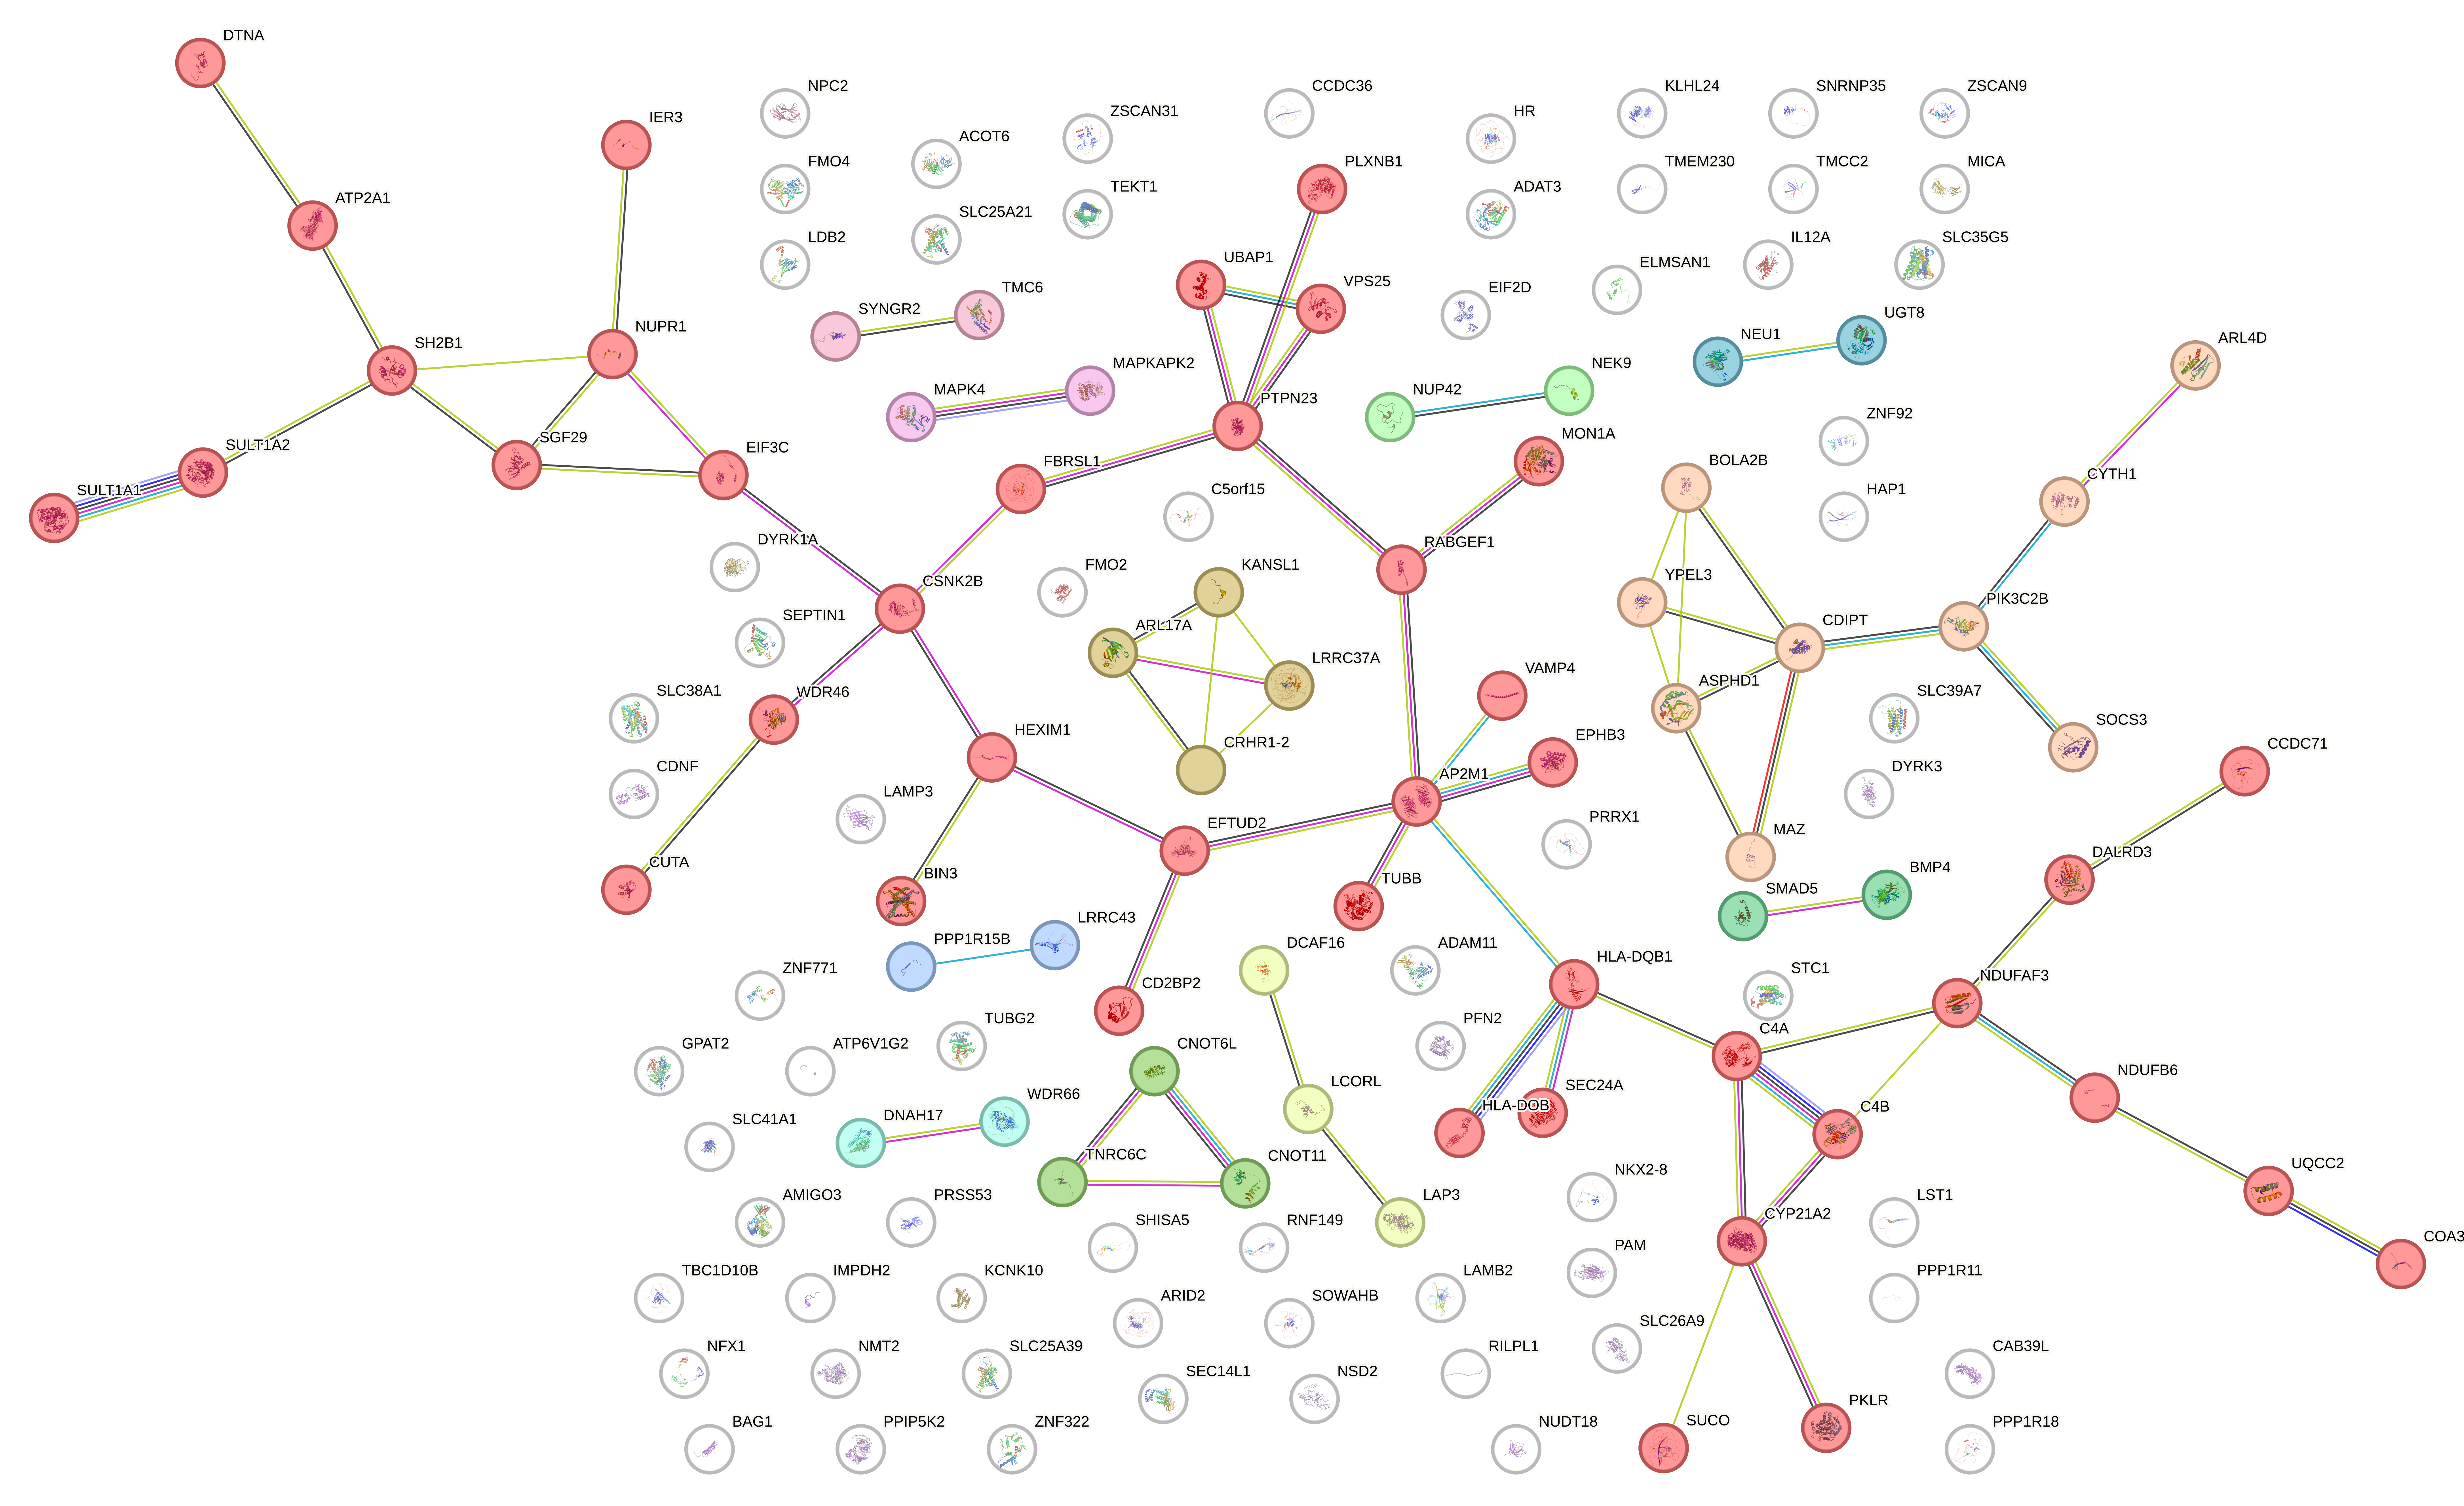
\includegraphics[width=1\linewidth]{Thesis/thesis images/network analysis.png}
    \caption{Network analysis showing connections between disease-eQTL-\textit{cis}-DEGs}
    \label{fig:enter-label}
\end{figure}
\end{landscape}
A network analysis of the eQTL-\textit{cis}-DEGs showed there were significantly more interactions than would be expected for a random set of proteins from both the genome ($p = 3.76e-08$) and from all \textit{cis}-genes ($p = 0.000677$). 
Additionally, there was a cluster of 41 genes (shown in red in figure X) that had significantly more interactions within the list of all 151 genes than expected ($p = 0.000775$). However, functional enrichment was only detected when comparing to the whole genome background. This indicates that whilst the list of eQTL-\textit{cis}-DEGs are more connected than expected, they do not cluster together within pre-defined pathways. NOT SURE ABOUT THIS STATEMENT which is concurrent with the GSEA results.



\section{Discussion}

strengths and limitations
future work
TADs?
conclusion
Talking
Non-identification of functional variants
Different study designs in the various databases used. In particular, the observational data from GEO and experimental data from PPMI 
Difficulty/effectiveness of common-variant/common-disease studies
The observed data from GEO is not restricted to just the SN. The SN is the smallest subsection of the samples. 
There is heterogeneity between each of the different experiments used from GEO, although there has been a lot of work by the lab to ensure the most comparable` datasets were used. 
This may impact which genes are differentially expressed.

Some talk about sQTL vs the eQTL


The GEO data is from tissue expression, so will include multiple cell types in the data. In contrast, the PPMI data is single cell.
There are were only 7 control samples available for the PPMI data, leaving it quite under-powered. When combined with the differing study designs between two expression datasets used, it becomes hard to draw robust conclusions from comparisons between the two. Since using the iPSC data was an attempt to both replicate and validate the expression in one step, it may be better to separate these, and replicate the heavy down-regulation of mitochondrial pathways observed in the GEO dataset using similar data first, then separately validate it.





\label{subsubsec:causality}


\section{Conclusion}


\bibliographystyle{unsrt}
\bibliography{Thesis/references.bib}
\end{document}


\subsubsection{Finding all SNPs in block ###DEPRECIATED???###}
The package LDlinkR's (citation) LDproxy function was used to extract the information for all variants in the database around each of the lead SNPs from the Nalls paper (citation) that were in high LD with the lead SNP (\(R^2\geq0.8\)). This generated a file that was then pruned with the physical coordinates of the LD block from section INSERTNUMBERHERE. The final output of this process was a file with INSERTNUMBERHERE variants, each tagged for which of the 88 LD blocks they came from. This failed for one of the lead SNPs (INSERTRSIDHERE), as it was classified as a functional variant, so proxies could not be found.

Initially, a preliminary analysis on the publicly accessible data in the GTEx database (citation) was completed. This was to ensure that usable results could be generated from the data. This preliminary search was targeted on the \textit{cis}-gene eQTL files provided, and specifically in the SN. This file was subsetted and combined with the file containing all the variants found within the LD blocks to generate a list of eGenes that were within 1mb of the variant and were significantly affected by it.

A total of 2650 (provisional number) genes within 1.5Mb of the disease loci were identified as being significantly affected (p\leq0.05) by at least one variant within the loci that was in high LD with the lead SNP, from the GTEx project data, in the SN. When the same process was applied to the BRAINEAC dataset, a total of ????? genes were identified. ???? genes were significant in both GTEx and BRAINEAC, and a total list of ????? was generated, which contained significant genes in either dataset. The number of significant genes for each block is displayed below:
TABLE????? SUMMARY INFORMATION